\documentclass{article}
\usepackage[utf8]{inputenc}
\usepackage{amsmath}
\usepackage{graphicx}
\usepackage{float}
\usepackage{geometry}
\usepackage{hyperref}
\hypersetup{
    colorlinks=true,
    linkcolor=blue,
    filecolor=blue,      
    urlcolor=blue,
    }

\title{BIM3007-Assignment1}
\author{Junyang Deng (120090791)}
\date{\today}
\geometry{left=3cm,right=3cm,top=2cm,bottom=2cm}
\begin{document} 
\maketitle

\section{Human genome project}

\begin{enumerate}
    \item[1.1] According to the most updated paper on the human genome released in April 2022 \cite{completegenome}, the size of human genome is 3.055 billion base pairs (bp). 
    The updated number of protein-coding region is around 19,969 protein coding genes. \\
    On average, a Chinese individual carries 3,068,811 SNVs and 257,832 INDELs, including 9106 missense variants, 10 stop loss, 73 stop gain, and 190 frameshift or non-frameshift INDELs, as reported by Westlake Biobank for Chinese (WBBC) in 2022 \cite{westlake}. 
    \begin{figure}[h]
        \centering
        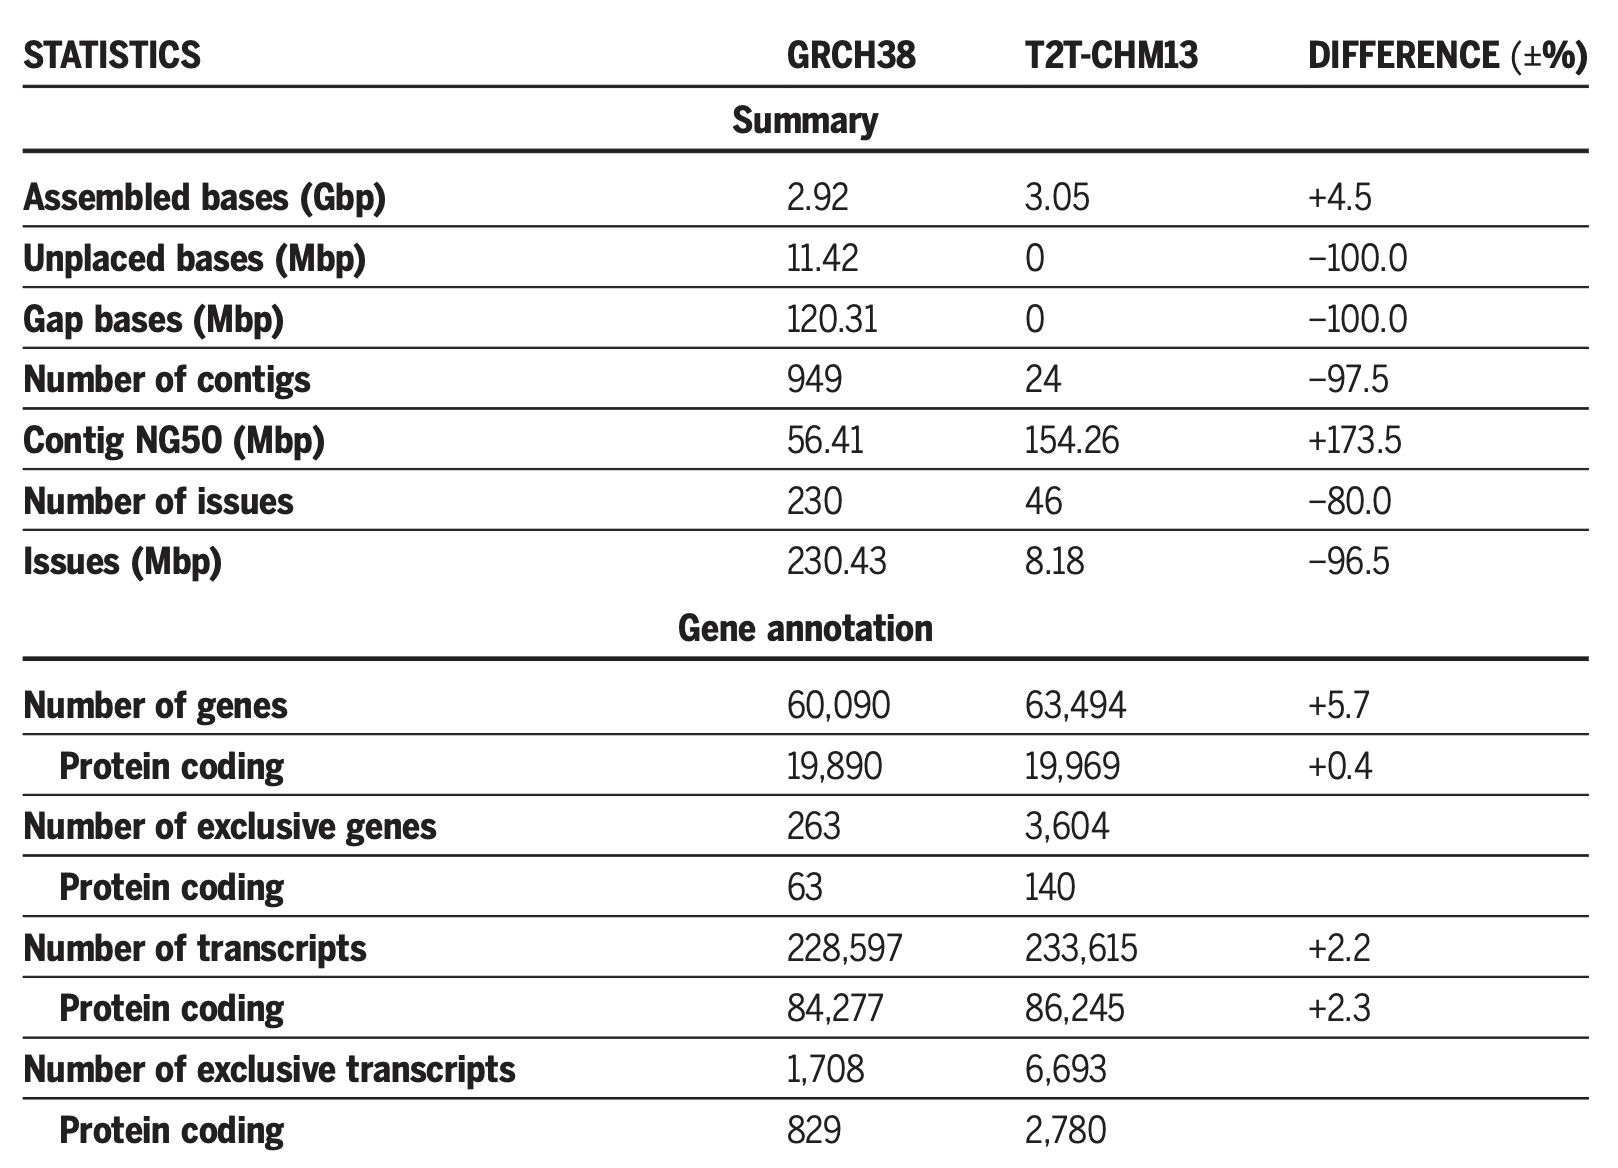
\includegraphics[scale=0.4]{A1-Image/comparison.png}
        \caption{Comparison between GRCH38 and T2T-CHM13}
    \end{figure}

    \item[1.2] The gene structure is illustrated in Figure \ref{genefig}. Usually, the transcription start site (TSS) denotes the beginning of gene. After TSS, there is a short segment called 5' untranslated region (UTR). The main body of gene primarily consists of two parts: exon and intron. Exons encode genes that will be translated to protein, while genes in intron region will be truncated during mRNA processing. At the end of the gene, there is a translation STOP codon, which is followed by 3' UTR. 
    \begin{figure}[h]
        \centering
        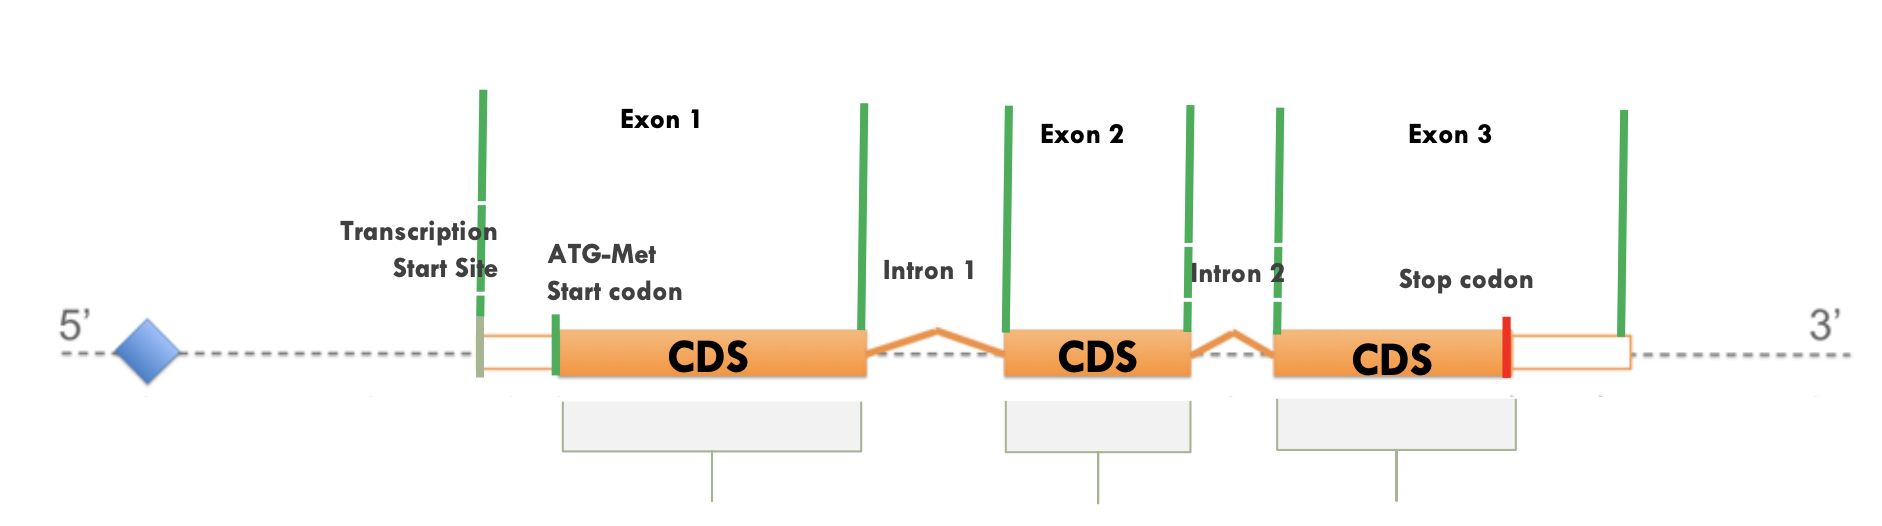
\includegraphics[scale=0.3]{A1-Image/Structure.png}
        \caption{Typical gene structure}
        \label{genefig}
    \end{figure}
    \item[ ] Genetic variants in different parts of gene exhibit different effects.
    \begin{itemize}
        \item Some mutations can affect the \textbf{presence} of a gene product. For example, if mutation occurs in the \textbf{regulatory region}, transcription factors can no longer bind to the sequence, and this will change the transcription status of gene. Similar consequences happen when missense occurs in start codon (\textbf{start loss}). This can also make the gene product disappear.
        \item Some mutations cause protein products to \textbf{malfunction}. Insertions, deletions, and nonsynonymous substitutions that happen in the genic area will change the composition of gene product. Whether or to what extend do genic mutation affect gene product depends on its location. If the mutation alters functional region of the gene product, the effect will be deleterious. If the mutation does not alter the functional region of the resulted protein, the effect will be more moderate.
        \item Some mutations, like synonymous mutations, have \textbf{no obvious effect} on gene products.
    \end{itemize}
\end{enumerate}
    
\section{Evolution of Sequencing technology}

\subsection{Principles of first, second, third generation sequencing technologies.}
\begin{description}
    \item[First generation] The first generation sequencing is also called Sanger sequencing. The procedure of Sanger sequencing is illustrated in Figure \ref{sanger}. First, dideoxynucleotide (ddNTP) are added to four tubes.  When ddNTP is incorporated into the DNA, DNA polymerase can no longer add nucleotides to the chain, and the synthesis will be terminated. ddNTPs used in the experiment are labelled by fluorescent dyes. Therefore, the result product of the first step will be DNA fragments of various length with ddNTP at the 3' end. Next, these fragments will be sent to run electrophresis. In electrophoresis, fragments will be sorted according to their length. Combining the location of fragments and the fluorescent color they exhibit, we can decode the sequence of interest. 
    \begin{figure}[h]
        \centering
        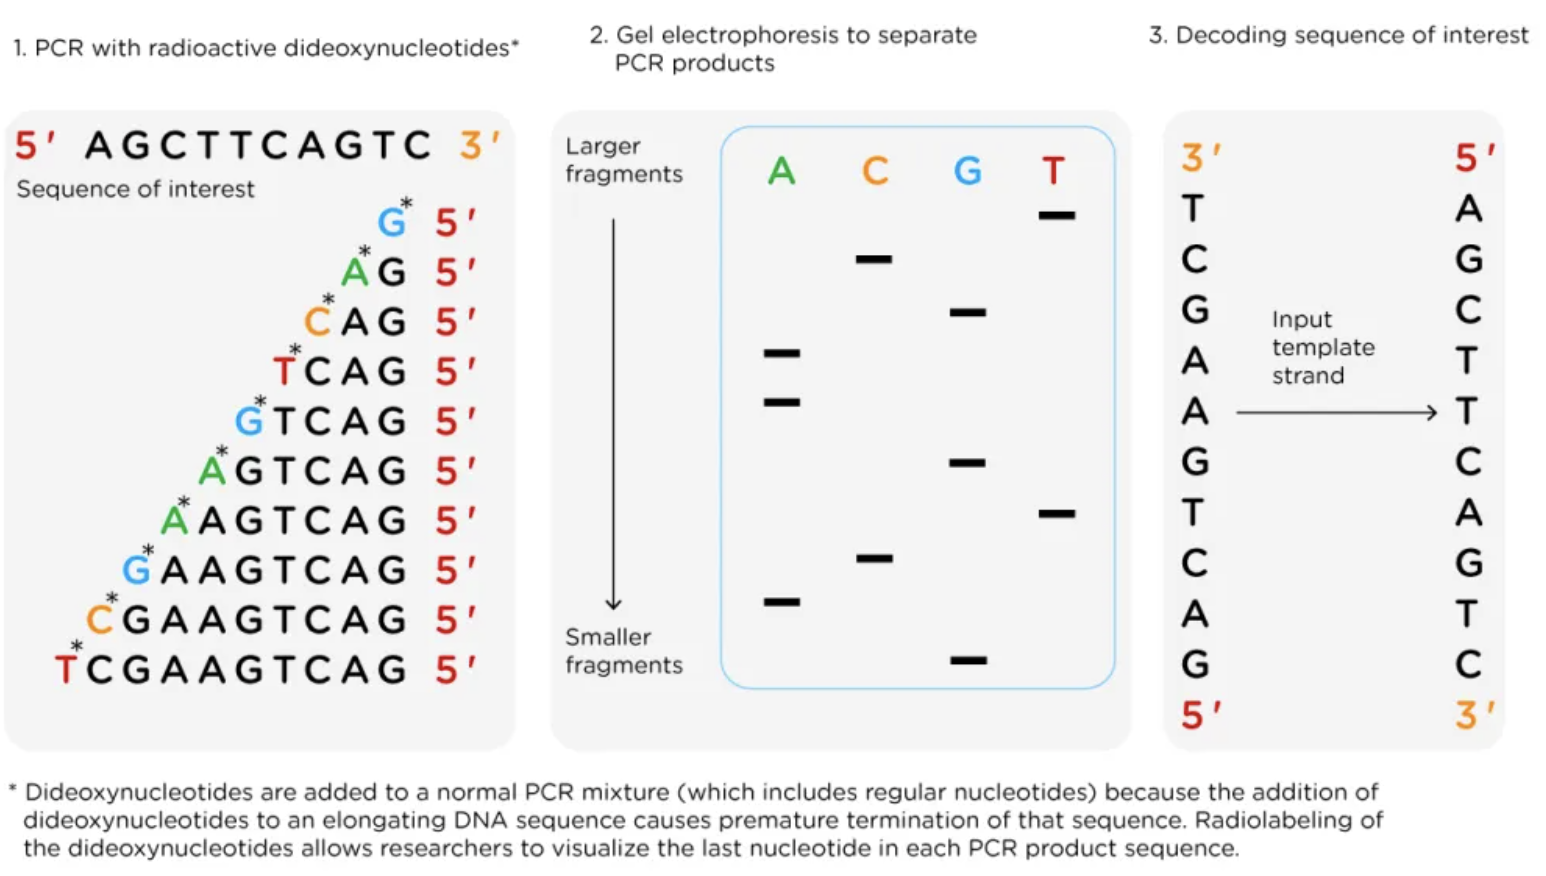
\includegraphics[width=\textwidth]{A1-Image/Sanger.png}
        \caption{Sanger Sequencing}
        \label{sanger}
    \end{figure}
    \item[Second generation] The second generation sequencing (also called next generation sequencing) is a high-throughput, parallel sequencing method. The main difference between first and second generation is that, second generation sequencing adopts modified dNTPs with fluorescently labelled terminator (not ddNTP anymore). When the labelled dNTP is incorporated in the sequence, the synthesis will be paused. Then, the machine will use laser to excite the fluorescent label, and synthesis can continue again. Similar to Sanger sequencing, the nucleotide can also be inferred from the color of fluorescent signal. To control the quality of reads, NGS has a bridge amplification process. Overall, the next generation sequencing method is much faster and more accurate than Sanger sequencing.
    \item[Third generation] The third generation is designed to read longer sequences in order to overcome the drawbacks of the first and second generation sequencing. Different companies are using fundementally different approaches to decode the DNA sequence. For example, Pacific Biosciences (PacBio) uses a Single-molecule real-time sequencing (SMRT-seq) method. This method detects the fluorescent signal right beside the DNA polymerase. Also, to ensure sequencing quality, circular consensus DNAs are formed. This allows the polymerase to sequence the fragments repeatedly \cite{ccs}. Different from PacBio, Oxford Nanopore technology (ONT) detects the change of current in the pore of nanoprotein. Compared to PacBio, ONT reads longer sequences but with a higher error rate.
\end{description}
\subsection{The pros and cons of different sequencing technologies.} 
    \begin{itemize}
        \item First generation
        \begin{itemize}
            \item pros: High accuracy
            \item cons: short read length (500 bp - 1,000 bp), time-consuming, labor-intensive, low throughput, cannot be used in highly repetitive region
        \end{itemize}
        \item Second generation
        \begin{itemize}
            \item pros: high-throughput, high accuracy (99.9\%), higher coverage, higher sequence depth, fast speed.
            \item cons: short read length (50 bp - 500 bp), cannot be used in highly repetitive region
        \end{itemize}
        \item Third generation
        \begin{itemize}
            \item pros: long read (usually tens of kbs fragments), can directly detect epigenetic modifications, suitable for de novo genome assembly \cite{hifi}.
            \item cons: lower accuracy (ONT 96\%, PacBio HiFi $>$ 99\%)
        \end{itemize}
    \end{itemize}


\section{Exome-sequencing data analysis}
\begin{itemize}
    \item[3.1] Exome includes all protein coding genes. Exome sequencing means to sequence the exome part of genome. The main goal of exome-sequencing technology is to figure out what loci are responsible for certain diseases at a relatively low cost. 
    \item[3.2] The process of Exome-sequencing data analysis includes three phases: raw data processing (denoising the data), variant calling, and integrative analysis.
    \item The first phase includes mapping, local realignment, duplicate marking, and base quality recalibration. The output will be analysis-ready reads. 
    \begin{itemize}
        \item Mapping: Raw sequencing data are many fragments of the sample DNA which includes replicates. So, the first step of analysing the reads is to map these short reads to a reference genome. (Software: \href{http://bio-bwa.sourceforge.net}{BWA} (Burrows-Wheeler Aligner))
        \item Local realignment: Some places are harder to alignment, for example indels. In order to improve the mapping quality, indel realignment is needed. In indel realignment, the software will first identify regions where realignments are needed. Then, reads in these regions will be realigned using a more accurate alignment strategy that takes all reads in the region into account.
        \item Duplicate marking: Fragments are duplicated during library construction. Before analysing the sequence, duplicates should be removed to avoid disturbance. (Software: Picard (by broadinstitude) (\href{https://github.com/broadinstitute/picard}{github codes}, \href{https://gatk.broadinstitute.org/hc/en-us/articles/360037052812-MarkDuplicates-Picard-}{introduction}))
        \item Base quality recalibration: Since sequencer might not procide the correct base quality score, we need to recalibrate it before variant calling. (Software: \href{https://gatk.broadinstitute.org/hc/en-us/articles/360035890531-Base-Quality-Score-Recalibration-BQSR-}{BQSR} (Base Quality Score Recalibration): A machine learning approach to recalibrate base quality scores. )
        \item After all these processes, analysis-ready reads will be generated. 
    \end{itemize}
    \item The second phase, variant calling phase, analyzes the alignment files to get variants. 
    \begin{itemize}
        \item There are three main types of variants: single nucleotide polymorphism (SNP), indel (insertion and deletion) and structural variant (SV). (Software: we can use \href{https://conifer.sourceforge.net/}{CoNIFER} to find copy number variants)
    \end{itemize}
    
    \item The third phase is integrative analysis. In this phase, external factors that can affect the variant calling result will be considered. With extra data, we can recalibrate variants and refine the genotype.
    \begin{itemize}
        \item For example, variants that lie in regions with bad mapping quality are less trustful than others. So as variants that lie in regions with low depth. A software called \href{https://gatk.broadinstitute.org/hc/en-us/articles/360035531612-Variant-Quality-Score-Recalibration-VQSR-}{VQSR} (Variant Quality Score Recalibration) can do this job. It is a sophisticated filtering technique applied on the variant callset that uses machine learning to model the technical profile of variants in a training set and uses that to filter out probable artifacts from the callset.
    \end{itemize}
\end{itemize}

\section{Exome-sequencing data analysis (application)}
% the pedigree tree
\begin{figure*}[h]
    \centering
    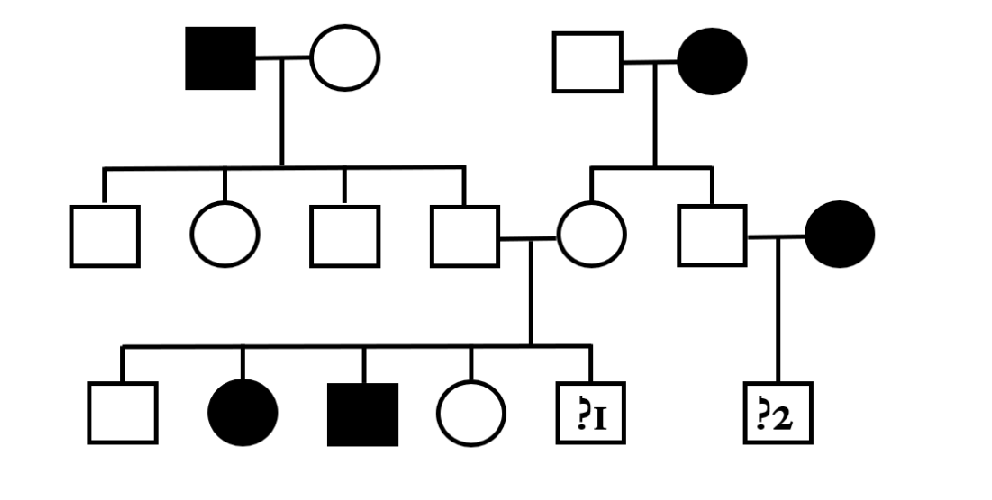
\includegraphics[scale=0.4]{A1-Image/Tree.png}
\end{figure*}

\begin{itemize}
    \item[4.1] The most likely inheritance is \textbf{autosomal recessive}. It is recessive because two patients appear in the third generation, but their parents are healthy individuals. It's also not X-linked recessive. If it is, II-6 must be ill because his mother passes a recessive gene to him.
    \item[4.2] The genotypes of child1's parents are Aa. So, the probability for them to have a diseased child is 1/4. As for the child2, his father's genotype must be Aa, so the probability of his disease is 1/2. 
    \item[4.3] Experiment design:
    \begin{enumerate}
        \item The first step of the experiment is to conduct sequencing on ill individuals. I will choose to sequence III-2 and III-3 because 1) this combination only involves 2 people thus the cost is low, 2) this disease is autosomal recessive, which requires two copies of genes to be recessive to get the disease. To reduce the search space, I choose people with lowest P(IBD=2) to sequence. In this case, the probability of IBD=2 is 1/4 for III-2 and III-3, which is the lowest of all.
        \item The second step is quality control. Data will go through the GATK pipeline (discussed in section 3.2). After that, a set of high quality variants are selected.
        \item Then, I will do sex examination and familial relation examination on the data. This can avoid false labeling of the samples. Sex is determined by calculating the homozygous ratio in X-chromosome. Familial relationship is estimated by calculating the pairwise IBDs among samples. 
        \item Next, we will filter out some variants based on variant frequency. In this step, we need to know the prevalence of this disease in the population. For instance, assume this disease has 100\% penetrance, if its prevalence is 0.01\%, the allele frequency should not be higher than 0.1\%.
        \item After that, we will follow the ACMG guideline to interpret the candidate variants \cite{ACMG}. The ACMG guideline combines computational (predicted) data, functional knowledge and clinical knowledge to help people understand the pathogenic effect of variants. This procedure can be completed using \href{https://github.com/WGLab/InterVar}{InterVar}.
    \end{enumerate}
    I followed the ACMG guideline to define the pathogenic variant. 
    The ACMG guideline uses typical types of variant evidence to classify variants into five categories --``pathogenic'', ``likely pathogenic'', ``uncertain significance'', ``likely benign'',and ``benign''. Typical types of variant evidence include population data (allele frequency), computational data (SIFT, PolyPhen, CADD), functional data (in vitro, in vivo), and clinical data (family history, segregation) etc. 

    The most important criterion for defining a pathogenic variant is the PVS1, which means a loss-of-function (LOF) mutation of a gene with known mechanism. Mutations that disrupt gene function by leading to a complete absence of gene products include nonsense, frameshift, canonical ±1 or 2 splice sites, initiation codon, single exon or multiexon deletion \cite{ACMG}. Once it is confirmed that the mutation is PVS1, the mutation will be classified as pathogenic or likely pathogenic, depending on whether it also meets other criteria.

    After finding out all the evidence, I can decide which category the variant belongs to. As shown in the Appendix, the combination of certain types of evidence can help decide the pathogenicity of the variant.
\end{itemize}

\section{GWAS}
\begin{table}[h]
    \centering
    \begin{tabular}{|l|l|l|l|}
        \hline
       & BB & Bb & bb \\ \hline
    AA & 23 & 51 & 34 \\ \hline
    Aa & 37 & 48 & 35 \\ \hline
    aa & 13 & 19 & 11 \\ \hline
    \end{tabular}
    \end{table}
\begin{itemize}
\item[5.1] Estimate the frquencies of the four haplotypes: AB, Ab, aB, ab using EM algorithm.
\begin{align*}
    \text{AB} &= 23 \times 2 + 51 + 37 = 134\\
    \text{Ab} &= 51 + 34 \times 2 + 35 = 154\\
    \text{aB} &= 37 + 13 \times 2 + 19 = 82\\
    \text{ab} &= 35 + 19 + 11 \times 2 = 76
\end{align*}

\begin{enumerate}
\item First iteration: 
    \begin{equation*}
    \begin{split}
        \text{P(AB and ab)} = 0.5\\
        \text{P(aB and Ab)} = 0.5
    \end{split}    
    \end{equation*}
    \begin{align*}
        \text{AB} &= 134 + 48\times 0.5 = 158, &~  f_{\text{AB}} = 158/542 = 0.2915\\
        \text{Ab} &= 154 + 48\times 0.5 = 178, &~  f_{\text{Ab}} = 178/542 = 0.3284\\
        \text{aB} &=  82 + 48\times 0.5 = 106, &~ f_{\text{aB}} = 106/542 = 0.1956\\
        \text{ab} &=  76 + 48\times 0.5 = 100, &~ f_{\text{ab}} = 100/542 = 0.1845
    \end{align*}
    \begin{align*}
       \text{P(AB and ab)} &= 0.2915 \times 0.1845 / (0.2915 \times 0.1845 + 0.3284 \times 0.1956) = 0.4557\\
       \text{P(Ab and aB)} &= 0.5443
    \end{align*}

\item Second iteration:
    \begin{align*}
        \text{AB} &= 134 + 48\times 0.4557 = 155.8736, &~ f_{\text{AB}} = 0.2876\\
        \text{Ab} &= 154 + 48\times 0.5443 = 180.1264, &~ f_{\text{Ab}} = 0.3323\\
        \text{aB} &= 82  + 48\times 0.5443 = 108.1264, &~ f_{\text{aB}} = 0.1995\\
        \text{ab} &= 76  + 48\times 0.4557 =  97.8736, &~ f_{\text{ab}} = 0.1806 
    \end{align*}
    \begin{align*}
        \text{P(AB and ab)} &= 0.4392\\
        \text{P(Ab and aB)} &= 0.5608
     \end{align*}
     \item Third iteration:
     \begin{align*}
        \text{AB} &= 134 + 48\times 0.4392 = 155.0816, &~ f_{\text{AB}} = 0.2861\\
        \text{Ab} &= 154 + 48\times 0.5608 = 180.9184, &~ f_{\text{Ab}} = 0.3338\\
        \text{aB} &= 82  + 48\times 0.5608 = 108.9184, &~ f_{\text{aB}} = 0.2010\\
        \text{ab} &= 76  + 48\times 0.4392 =  97.0816, &~ f_{\text{ab}} = 0.1791 
    \end{align*}
    \begin{align*}
        \text{P(AB and ab)} &= 0.4331\\
        \text{P(Ab and aB)} &= 0.5669
    \end{align*}     
\item Fourth iteration:
    \begin{align*}
       \text{AB} &= 134 + 48\times 0.4331 = 154.7888, &~ f_{\text{AB}} = 0.2856\\
       \text{Ab} &= 154 + 48\times 0.5669 = 181.2112, &~ f_{\text{Ab}} = 0.3343\\
       \text{aB} &= 82  + 48\times 0.5669 = 109.2112, &~ f_{\text{aB}} = 0.2015\\
       \text{ab} &= 76  + 48\times 0.4331 =  96.7888, &~ f_{\text{ab}} = 0.1786 
    \end{align*}
    \begin{align*}
        \text{P(AB and ab)} &= 0.4309\\
        \text{P(Ab and aB)} &= 0.5691
    \end{align*}
\item Fifth iteration:
    \begin{align*}
        \text{AB} &= 134 + 48\times 0.4309 = 154.6832, &~ f_{\text{AB}} = 0.2854\\
        \text{Ab} &= 154 + 48\times 0.5691 = 181.3168, &~ f_{\text{Ab}} = 0.3345\\
        \text{aB} &= 82  + 48\times 0.5691 = 109.3168, &~ f_{\text{aB}} = 0.2017\\
        \text{ab} &= 76  + 48\times 0.4309 =  96.6832, &~ f_{\text{ab}} = 0.1784 
    \end{align*}
    \begin{align*}
        \text{P(AB and ab)} &= 0.4300\\
        \text{P(Ab and aB)} &= 0.5700
    \end{align*}
\end{enumerate}

\item[5.2] Describe whether the two SNPs are in linkage disequilibrium.

The allele frequencies and the estimated haplotype frequencies (from EM-algorithm) are shown in Table 1 and 2.
\begin{table}[h!]
    \centering
    \begin{tabular}{|l|l|}
    \hline
    haplotype & Frequency \\ \hline
    AB        & 0.2854    \\ \hline
    Ab        & 0.3345    \\ \hline
    aB        & 0.2017    \\ \hline
    ab        & 0.1784    \\ \hline
    \end{tabular}
    \caption{Estimated haplotype frequencies}
\end{table}

\begin{table}[h!]
    \centering
    \begin{tabular}{|l|l|}
    \hline
    Allele & Frequency \\ \hline
    A      & 0.6199    \\ \hline
    a      & 0.3801    \\ \hline
    B      & 0.4871    \\ \hline
    b      & 0.5129    \\ \hline
    \end{tabular}
    \caption{Estimated allele frequencies}
\end{table}

\begin{align*}
    & D = P(AB) - P(A)P(B) = 0.2854 - 0.6199 \times 0.4871 = -0.0166\\
    & D_{\text{max}} = - P_a P_b = -0.3801 \times 0.5129 = -0.1950\\
    & D' = D/D_{\text{max}} = 0.0166/0.1950 = 0.0851\\
    & R^2 = D^2/(P_A P_B P_a P_b) = 0.0166^2/(0.3801 \times 0.5129 \times 0.6199 \times 0.4871) = 0.0047
\end{align*}
Since $R^2$ is less than 0.1, the two SNPs are likely independent (not in linkage disequilibrium).
\end{itemize}

\section*{Appendix}
The ACMG guidelines for reporting of incidental findings in clinical exome and genome sequencing \cite{ACMG}.

Pathogenic:
\begin{enumerate}
    \item 1 Very strong (PSV1) AND
    \begin{enumerate}
        \item $\geq$ 1 Strong (PS1-PS4) OR 
        \item $\geq$ 2 Moderate (PM1-PM6) OR
        \item 1 Moderate (PM1-PM6) and 1 supporting (PP1-PP5) OR
        \item $\geq$ Supporting (PP1-PP5)
    \end{enumerate}
    \item $\geq$ 2 Strong (PS1-PS4) OR
    \item 1 Strong (PS1-PS4) AND
    \begin{enumerate}
        \item $\geq$ 3 Moderate (PM1-PM6) OR
        \item 2 Moderate (PM1-PM6) AND $\geq$ Supporting (PP1-PP5) OR
        \item 1 Moderate (PM1-PM6) AND $\geq$ 4 Supporting (PP1-PP5)
    \end{enumerate}
\end{enumerate}

\bibliographystyle{unsrt}
\bibliography{reference}

\end{document}
